\newasm{
For charged current quasielastic scattering of a neutrino with a free nucleon,
the interaction is described by a $V-A$ weak interaction given at the quark level by
$\bar{u}\gamma_\mu(1- \gamma_5)d$ (or its conjugate), with the nucleon level amplitude at four-momentum transfer $Q^2 = -q^2$ described by
\begin{align}
 \langle p | V^\mu | n \rangle
 &= \bar{u}_p \Big[
 F_1(q^2) \gamma^\mu +\frac{i}{2M} F_2(q^2) \sigma^{\mu\nu} q_\nu
 \Big] u_n,
 \nonumber\\
 \langle p | A^\mu | n \rangle
 &= \bar{u}_p \Big[
 F_A(q^2) \gamma^\mu \gamma_5 +\frac{1}{M} F_P(q^2) q^\mu \gamma_5
 \Big] u_n\, .
\end{align}
Existing calculations from LQCD extend up to a range of $Q^2 \lesssim 1~{\rm GeV}^2$,
which is ideal for the neutrino interactions at the ${\rm GeV}$ energy scale.
}

{\color{red}TRANSPLANTED FROM OLD INTRO}
For example, Figure~\ref{fig:protonmagneticff} demonstrates the current tension in the determination of the proton magnetic form factor.
Two different parameterizations of the form factor, normalized by the dipole are displayed.
The Bradford, Bodek, Budd and Arrington parameterization from Neutrino-Nucleus Interaction 2005 Workshop (BBBA05)~\cite{Bradford:2006yz} are displayed as the lower (blue) band with a solid mean value.
A more recent z-expansion parameterization from Borah {\it et al.}~\cite{Borah:2020gte} is displayed by the upper (black) band with a dashed mean value.
Of note, even the sign of the slope of the form factor is not determined.

\newasm{
The vector form factors, $F_1$ and $F_2$,
are precisely estimated from electron-proton scattering data,
up to a tension in existing parameterizations of the proton magnetic form factor
shown in Fig.~\ref{fig:protonmagneticff}.
The tension is significant over all $Q^2 > 0$, at the level of several percent,
including significant disagreement in the slope of the form factor at $Q^2 = 0$.
Of the nucleon form factor calculations from lattice QCD,
the vector form factors are also the most mature,
exhibiting no obvious tensions with experimental determinations
of the vector form factors at the level of the lattice precision.
\textcolor{red}{[what percent precision?]}
A percent level calculation of the form factor $Q^2$ behavior
or a direct calculation of the slope of the magnetic form factor
would provide useful insight about this tension or could discriminate
between the two parameterizations.
}

%------------------------------------------------------------------------------
% proton magnetic FF
\begin{figure}[hbt!]
 \centering
 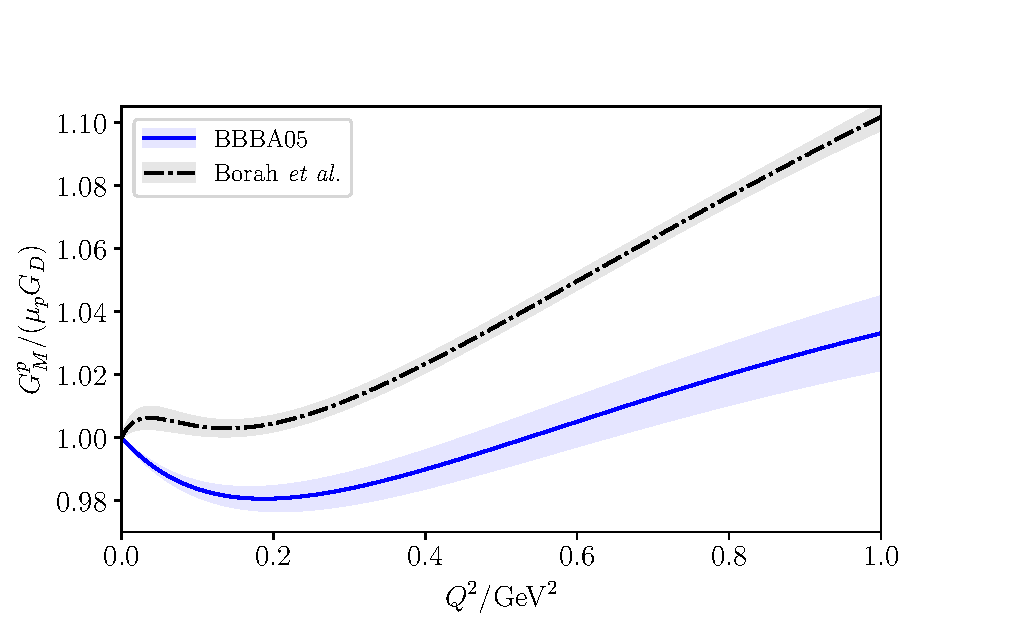
\includegraphics[width=0.75\textwidth]{plots/proton_magnetic-standalone.pdf}
\caption{
Proton magnetic form factor normalized by a reference dipole ansatz
with a dipole mass of $0.84~{\rm GeV}$.
The proton-only fit to a $z$ expansion by Borah {\it et al.}~\cite{Borah:2020gte}
and the BBBA05 parameterization~\cite{Bradford:2006yz} are shown.
\label{fig:protonmagneticff}
}
\end{figure}
%------------------------------------------------------------------------------



\newasm{
The nucleon axial form factor has had a much more complicated past
 than the vector form factors in lattice QCD.
The axial charge, the value of the axial form factor at $Q^2=0$,
 is a key benchmark for lattice QCD and is precisely known
 from neutron decay experiments.
LQCD calculations of the axial charge have historically been low compared
 to experiment, and the discrepancy has been the topic of some controversy.
As treatment of systematics have become more sophisticated,
 modern calculations of the axial charge have finally started to come into
 agreement with the experimental value at the percent level.
}

\newasm{
Armed with the newfound confidence in the control of systematics for the axial charge,
 more emphasis is now being put into the form factor at nonzero momentum transfer.
One extremely striking feature of lattice calculations is the strong preference for a slower
 fall off of the form factor with increasing $Q^2$ than predicted by experiment.
This preference is consistently reproduced by several lattice collaborations using
 independent computation methods, lending more credence to the result.
When integrated over the full range of $Q^2$ to compute the nucleon cross section,
 this translates to an enhancement in the free nucleon cross section as large as $30-40\%$
 over neutrino energies greater than $1~{\rm GeV}$.
In addition, the precision on the axial form factor uncertainty from lattice QCD
 is small enough to be sensitive to the tension between vector form factor parameterizations.
}

\newasm{
The aformentioned situation with nucleon form factors
 is depicted in Fig.~\ref{fig:nucleonxsec}.
The black dot-dashed curve is the default case,
 which uses the $z$ expansion parameterizations of the vector and axial
 form factors from Refs.~\cite{Borah:2020gte}~and~\cite{Meyer:2016oeg}, respectively.
The green band shows the uncertainty obtained from the axial form factor alone,
 and the gray band from the (much smaller) vector form factor uncertainty by itself.
The blue solid curve substitutes the vector form factors of the default choice
 with the BBBA05 parameterization~\cite{Bradford:2006yz},
 taking the uncorrelated uncertainty from the BBBA05 vector form factors only.
The observed tension between the black and blue bands is the result of the
 tension between proton magnetic form factor parameterizations.
The red dotted curve instead substitutes the axial form factor of the default
 with a parameterization obtained from lattice QCD and its uncertainty.
The size of the red band with respect to the green band demonstrates
 the uncertainty reduction from replacing the deuterium scattering
 axial form factor with one obtained from LQCD,
 and the significant change in normalization is due to the slower fall off
 of the axial form factor.
Additionally, the size of the red band demonstrates the relevance
 of the tension in vector form factors, characterized by the difference
 between the black and blue curves.
}


%------------------------------------------------------------------------------
% nu-N cross section
\begin{figure}[hbt!]
 \centering
 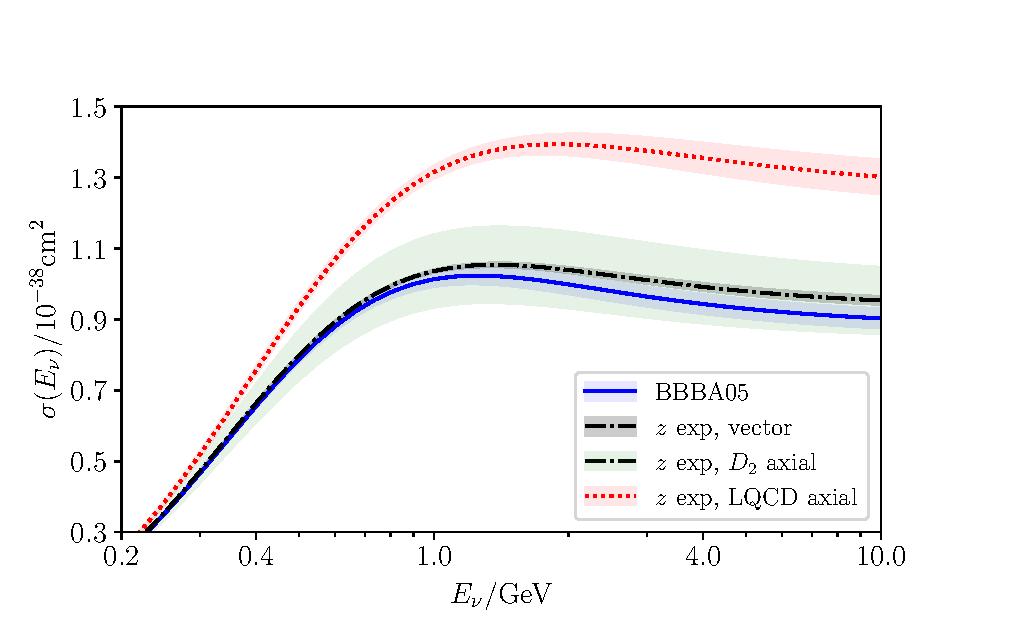
\includegraphics[width=0.75\textwidth]{plots/xsec_comparison-standalone.pdf}
\caption{
 Neutrino cross sections on a free neutron, with their uncertainty bands,
 for various choices of parameterization.
 The curves labeled ``BBBA05'' (blue solid line, Ref.~\cite{Bradford:2006yz})
 and ``$z$ exp, vector'' (black dot-dashed line, Ref.~\cite{Borah:2020gte}) use the
 $z$ expansion axial form factor from Ref.~\cite{Meyer:2016oeg},
 with only the uncertainty from the vector form factors plotted
 to highlight the tension between the parameterizations shown in Fig.~\ref{fig:protonmagneticff}.
 The same form factor parameterizations are used for both ``$z$ exp, vector'' and
 ``$z$ exp, $D_{2}$ axial'' (green dot-dashed line)
 but in the latter case the uncertainty band is taken only from
 the axial form factor rather than only from the vector form factor.
 The red dotted line labeled ``$z$ exp, LQCD axial'' is parameterized by
 the vector form factors of Ref.~\cite{Borah:2020gte} with no uncertainty
 and the axial form factor with its uncertainty taken from LQCD.
 \label{fig:nucleonxsec}
}
\end{figure}

\newasm{
So far, the focus of this manuscript has been on the charged-current
 quasielastic form factors, which are the easiest target for lattice QCD
 efforts and most relevant to the next-generation neutrino oscillation program.
Of these, the axial form factor has gotten the most attention from lattice collaborations
 and is the focus of the material in Sec.~\ref{sec:lqcd}.
The phenomenological impact of the axial form factor obtained from lattice QCD
 is given in more detail in Sec.~\ref{sec:impact}.
}

\newasm{
Similar calculations could also access the isoscalar form factors of the nucleon,
 which apply to neutral current scattering amplitudes,
 although the precision obtained from these calculations is more limited
 due to the sensitivity of the measurement to the background gauge fields
 in the lattice gauge configurations.
More challenging computations could provide information about nucleon
 resonant and nonresonant contributions to axial matrix elements,
 such as the $\Delta$ or Roper resonance channels,
 inclusive contributions in the shallow inelastic scattering region,
 or deep inelastic scattering parton distribution functions.
Some applications of lattice QCD to other interaction mechanisms
 are outlined in Sec.~\ref{sec:future}.
}

\begin{description}
\item[first $z$ exp vector form factor] \cite{Ye:2017gyb}
 - does not use constraints from muonic hydrogen, many more fit parameters
\item[Vector form factor tensions] \cite{Borah:2020gte}
\item[Muonic hydrogen review] \cite{Hill:2017wgb}
\end{description}

\textcolor{red}{[Most focus on axial, but vector is important too]}
